\chapter{Metodologia}

No desenvolvimento de um projeto, o planejamento do método a ser utilizado
é essencial para a boa qualidade da execução. No projeto UMISS, o método
utilizado em diferentes áreas do conhecimento foi planejada e pensada;
este capítulo levantará os métodos e definições utilizadas pelo grupo.

\section{Estrutura Analítica do Projeto (EAP)}
A Estrutura Analítica do Projeto (EAP) é a decomposição hierárquica do escopo 
toral do trabalho a ser executado pela equipe do projeto a fim de alcançar
os objetivos do projeto e criar as entregar exigidas. Cada nível descendente 
da EAP representa uma definição cada vez mais detalhada do trabalho do 
projeto. \cite{pmbok}.

A partir dessa definição foi criada uma EAP, representada na figura \ref{fig:eap}
para o presente projeto, realizando 
a divisão das entregas de acordo com o exigido nos pontos de controle da 
disciplina Projeto Integrador 2.

\begin{figure}[H]
  \centering
    \includegraphics[width=\textwidth]{figuras/eap-umiss-3.eps}
  \caption{Estrutura Analítica de Projeto}
  \label{fig:eap}
\end{figure}

\section{Comunicação}

Para a gestão de grandes equipes, uma comunicação efetiva é essencial e de extrema importância.
Esse cuidado pode garantir o sucesso do projeto, de modo contínuo, desde o planejamento até
a integração dos subsistemas.
O grupo, na elaboração do projeto UMISS, utilizou o Slack\footnote{\url{https://slack.com/}}
para comunicação geral; o Google Drive para armazenamento e atividades conjuntas; o Github para mapeamento
das atividades a serem feitas e o Google Hangouts para reuniões remotas. Além disso, reuniões
periódicas foram feitas com os integrantes do grupo, principalmente para tratar assuntos
que precisassem da presença de todos.

\section{Tempo}

Para gerenciar o tempo no projeto, foi utilizado como base os processos
de gerenciamento de tempo do \cite{pmbok2012}.

A partir do escopo do projeto, foi feito o cronograma inicial utilizando o software Gantter armazenado no Google Drive para que todos os membros do projeto
possam acessá-lo e assim fazer o controle do cronograma.

\subsection{Cronograma}

O cronograma encontra-se no Apêndice \ref{schedule_appendix}.

\section{Recursos Humanos}

O projeto foi dividido em três subsistemas, que são: Processamento de Sinais e Monitoramento,
Projeto Estrutural e Controle e Alimentação. Dentro dos subsistemas a equipe
técnica foi dividida de acordo com a demanda de cada área e levando em conta o
conhecimento prévio de cada integrante, bem como o seu interesse de atuação. Os
subsistemas serão gerenciados por um Gerente Geral, um Gerente de Qualidade e
um Gerente de Produto.
Abaixo tem-se uma breve descrição do setor de gerenciamento e dos subsistemas,
e também os integrantes que compõem cada área. É válido ressaltar que a
distribuição e responsabilidades de cada equipe poderão sofrer mudanças no
decorrer do projeto para melhor atender as necessidades de cada área e
consequentemente obter um melhor desempenho dos integrantes e o êxito do projeto.

\subsection{Gerenciamento}

\textbf{Gerente Geral:} responsável pelo planejamento, pela organização e pelo controle das atividades desempenhadas pelos integrantes de cada equipe, bem como pela assessoria a cada subsistema e atualização de informações pertinentes ao projeto como um todo.
\\Responsável: Afonso Delgado

\textbf{Gerente de Qualidade:} responsável por fiscalizar a qualidade do que está sendo produzido fazendo uma análise crítica da produção, de maneira a obter uma maior confiabilidade, produtividade, redução de custos e otimização dos processos realizados por cada equipe.
\\Responsável: Dylan Guedes

\textbf{Gerente de Produto:} responsável por prestar suporte a todos os subsistemas, visando aperfeiçoar a capacidade de produção dos integrantes do projeto, focando na qualidade da entrega final, impedindo, assim,  que fatores alheios atrapalhem a experiência do cliente com o produto final.
\\Responsável: Rafael Amado

\subsection{Subsistemas}

\textbf{Processamento de Sinais e Monitoramento:} responsável pela aquisição de sinais vitais do paciente,
tratamento de sinais, amplificação e conversão, transmissão e apresentação de
dados via notificações web e mobile.
\\Responsáveis: Dylan Guedes, Wilton Rodrigues, Tiago Assunção, Gustavo Cavalcante e Afonso Delgado.

\textbf{Projeto Estrutural:} responsável pelo projeto estrutural da cadeira, testes
do sistema estrutural, simulações e construção da cadeira.
\\Responsáveis: Nivaldo Lopo, Rafael Amado, Lucas Oliveira.

\textbf{Controle e Alimentação:} responsável por dimensionamento dos motores utilizados,
baterias e sistemas de movimentação e ativação dos motores (controle por
joystick e driver para motores).
\\Responsáveis: Lunara Martins, Mariana Andrade, Cesar Marques, Johnson Andrade e Felipe Costa.

Na Figura \ref{fig:flux_rh} é apresentada a estrutura de alocação de recursos humanos da equipe.


\begin{figure}[h]
    \centering
    \includegraphics[keepaspectratio=true,width=\textwidth]{figuras/rh-umiss.eps}
    \caption{Estrutura de alocação de recursos humanos.}
    \label{fig:flux_rh}
\end{figure}

\subsection{Tarefas}

As tarefas feitas por cada membro foram condensadas em tabelas apresentadas no apêndice \ref{app:tarefas}.


\section{Desenvolvimento do Relatório}

A confecção do relatório será dividida em dois fluxos - um geral, onde o
conteúdo será escrito e revisado, e a implantação no relatório, onde um
membro que domine \LaTeX\ e
Git\footnote{\url{https://git-scm.com/}} transcreverá o conteúdo para o
relatório final.

\subsection{Fluxo 1 - Criação do conteúdo}

\begin{figure}[H]
  \centering
    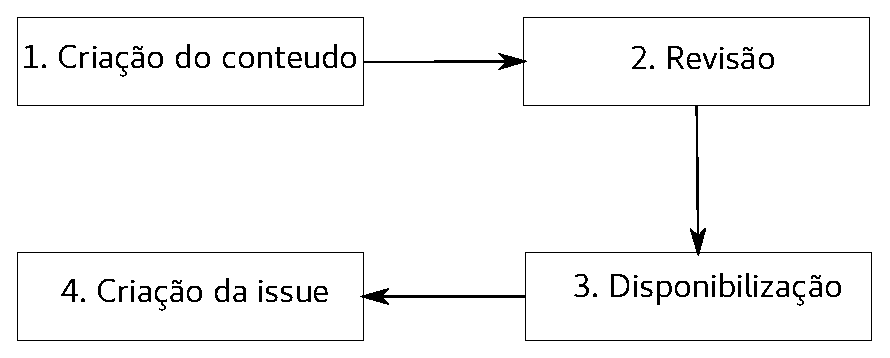
\includegraphics[width=\textwidth]{figuras/fluxo1.eps}
  \caption{Fluxo 1 - Criação do conteúdo.}
  \label{fig:fluxo1}
\end{figure}

\begin{enumerate}
  \item O conteúdo é escrito, de maneira formatada e com referências;
  \item O conteúdo é revisado pelo seu autor, que corrigirá defeitos encontrados;
  \item O autor disponibiliza o conteúdo em algum meio acessível pelos outros membros;
  \item O autor cria uma \textit{issue} no repositório do
    relatório\footnote{\url{https://github.com/CadeiraCuidadora/relatorio}}, explica brevemente
    o conteúdo criado, e disponibiliza o \textit{link} para o conteúdo. A \textit{issue} deverá ser associada a \textit{label} de relatório.
\end{enumerate}

\subsection{Fluxo 2 - Implantação no Relatório}

\begin{enumerate}
  \item Um membro que domine Git e \LaTeX\ encontra uma \textit{issue} que deseja
  implantar no relatório;
  \item Revisa o conteúdo, e o transcreve para o relatório;
  \item Relata na \textit{issue} associada se algum problema ocorreu, ou se terminou a transcrição;
  \item Cria um \textit{merge request} para a \textit{branch master} no repositório;
  \item Outro membro revisa o \textit{merge request}, e aceita ou relata as correções a serem feitas.
\end{enumerate}

